\label{chap.9}
\section{Introduction}
The prototype is \emph{Slice Twin}, a monitor that runs in the browser and shows how different controllers split the bandwidth of each cell between eMBB, URLLC and mMTC over one day of real Milan traffic. It makes the environment of Chapter~\ref{chap.4} and the experiments of Chapters~\ref{chap.7} and~\ref{chap.8} something you can click through. The source is in \texttt{app/slice\_twin} of the project repository, and the monitor, a results dashboard and a project brief are published at \texttt{https://fyp-a09.github.io/6G/}.

\section{Purpose and Design}
Slice Twin lets you watch what the controllers do, see how incidents hit each slice, and compare forecast-based allocation with simpler allocation on the same data.

\paragraph{Data shown.}
One held-out day is replayed: Wednesday 6 November 2013, which the forecaster was not trained on (days 5 and 6 are excluded from its training for this reason). The traffic is real Telecom Italia Milan data \cite{barlacchi2015}. We inject scripted incidents so that the controllers have something to react to: an mMTC storm, an interference spike, a cell outage, a backhaul degradation, a flash crowd and a URLLC burst on the central block. The city view adds four more, namely a firmware push in the north-west, wide-area interference in the east, storm damage in the south and a crowd at San Siro. Every incident is labelled and described in the interface. They are scripted for the demonstration and are not real events.

\paragraph{Interaction model.}
The interface is modelled on Cisco Packet Tracer. In Realtime mode the day plays continuously at a speed you choose. In Simulation mode the playback stops at each new event. An event list gives the time, cells and description of every incident, and a timeline marks the incidents and lets you jump to any time of the day.

\section{Views and Controllers}
\label{sec:slice-views}
\paragraph{Block view.} The 100 central cells ($10\times10$) are drawn as rings. The segments of a ring show how the cell splits its capacity between the three slices, and moving packets show the traffic that is served. Selecting a cell opens an inspector with its demand, its allocation, its latency against the target and the SLA status of each slice.

\paragraph{City view.} All 10{,}000 cells are drawn as a map that can be coloured by real traffic, by load or by SLA misses, with landmarks (Duomo, Milano Centrale, San Siro, Linate airport, Navigli, Citt\`a Studi) and the active incidents. Selecting a cell compares the three controllers on it over the day, and a cell of the central block can be opened in the block view. City-wide curves show the bandwidth given to each slice and the fraction of cells meeting each SLA, with an option to show the gain over the Reactive controller.

\paragraph{Controllers.} Three controllers run in the same environment (Chapter~\ref{chap.4}).
\begin{itemize}
	\item \textbf{Static:} an equal split of each cell's capacity that never changes.
	\item \textbf{Reactive:} the expert rule, which gives URLLC and mMTC enough capacity to stay under their SLA-safe utilisation and the rest to eMBB, using the current demand.
	\item \textbf{Predictive:} the same rule fed with the TGNN forecast of the next ten minutes (the city-trained forecaster of Chapter~\ref{chap.6} in the city view).
\end{itemize}
These are the controllers of Section~\ref{sec:city-controllers}, so the monitor agrees with Table~\ref{tab:city-controllers}. On the central block (Table~\ref{tab:block-controllers}) the Predictive controller is better than Reactive, and an oracle that knows the true next demand would be better still. Over the whole city the Static split scores highest.

\begin{table}[htbp]
\centering
\caption{Controllers on the 100 central cells, Wednesday 6 November 2013}
\label{tab:block-controllers}
\footnotesize
\begin{tabular}{|>{\centering\arraybackslash}p{\dimexpr 0.300\textwidth-2\tabcolsep\relax}|>{\centering\arraybackslash}p{\dimexpr 0.170\textwidth-2\tabcolsep\relax}|>{\centering\arraybackslash}p{\dimexpr 0.170\textwidth-2\tabcolsep\relax}|}
\hline
\textbf{Controller} & \textbf{SLA met (eMBB / URLLC / mMTC)} & \textbf{Reward} \\ \hline
Static & 0.13 / 0.98 / 1.00 & 0.709 \\ \hline
Reactive & 0.59 / 0.74 / 0.57 & 0.735 \\ \hline
Predictive & 0.59 / 0.82 / 0.61 & 0.768 \\ \hline
Oracle (true next demand) & 0.59 / 1.00 / 1.00 & 0.876 \\ \hline
\end{tabular}
\end{table}

\section{Technical Notes}
\label{sec:slice-tech}
\paragraph{Technology and data flow.}
Slice Twin is a static web application with no code on a server. All the calculations are done beforehand, and the browser (HTML, CSS and JavaScript) only reads the prepared files and draws the views (Figure~\ref{fig:slice-flow}).
\begin{figure}[htbp]
	\centering
	\small
	\fbox{\parbox{0.92\textwidth}{\centering
	Milan traffic $\rightarrow$ unified environment $\rightarrow$ three controllers with incidents and forecast (Python, offline)\\
	$\downarrow$\\
	\texttt{data.json} (block), \texttt{city.json} and \texttt{city.bin.gz} (city)\\
	$\downarrow$\\
	Browser reads the files and draws the views and charts}}
	\caption{Data flow of the Slice Twin monitor}
	\label{fig:slice-flow}
\end{figure}
The files are produced by \texttt{showcase.py} for the block view and \texttt{showcase\_city.py} for the city view, both in \texttt{src/unified}. The city data is stored compactly. For each interval and cell, one byte holds the log-scaled demand. For each controller, one byte holds the load (scaled by 250) and one byte holds flags: bits 0 to 2 say whether each slice meets its SLA, bit 3 marks an event and bit 4 an outage. The compressed binary file is a few megabytes, so the browser can handle 10{,}000 cells over 144 intervals and three controllers.

\paragraph{How to run it.}
From the root of the repository, \texttt{python -m http.server 8765 --directory app/slice\_twin} starts the monitor at \texttt{http://localhost:8765}. To regenerate the data, run \texttt{showcase.py}, then \texttt{forecast\_\allowbreak city\_\allowbreak v2.py} once to train the city forecaster, and then \texttt{showcase\_\allowbreak city.py}; the Milan files must be on the project drive. A GitHub Actions workflow publishes the monitor, the results dashboard and the project brief to GitHub Pages whenever the site or monitor folders change.

\paragraph{Demonstration.}
Figure~\ref{fig:slice-city} shows the city view at 17:30 on the demonstration day. In the top image the cells are coloured by real traffic, with the storm-damage incident in the south marked, and in the bottom image by SLA misses under the Reactive controller.
\begin{figure}[htbp]
    \centering
    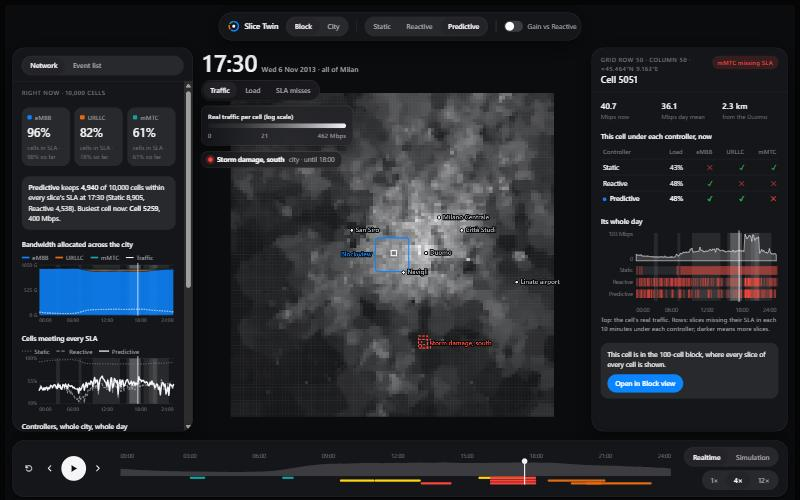
\includegraphics[width=0.92\textwidth]{slice_twin_city_dark.jpg}\\[1.2em]
    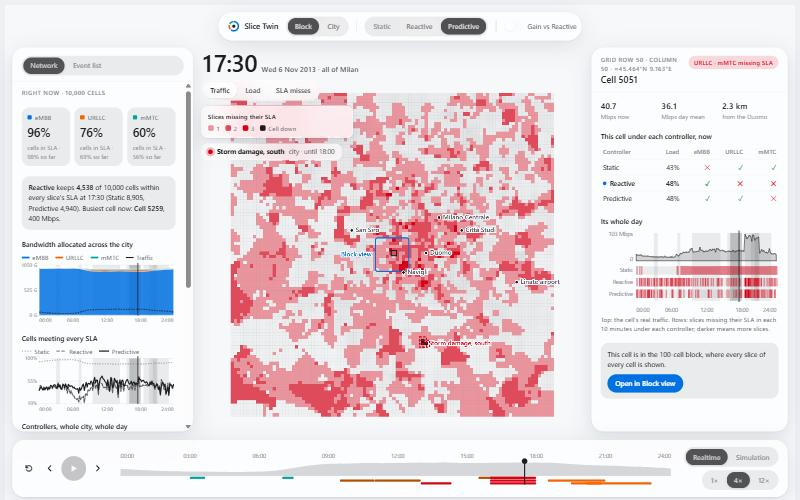
\includegraphics[width=0.92\textwidth]{slice_twin_city_light.jpg}
    \caption{City view at 17:30: cells coloured by real traffic (top, dark theme) and by SLA misses under the Reactive controller (bottom, light theme).}
    \label{fig:slice-city}
\end{figure}

\section{Contribution to the Project}
\label{sec:slice-contrib}
The Slice Twin monitor is the working product of the project, and the code, the unified environment and the dataset in the repository stand behind it. It also works as a demonstration. A viewer can see that the predictive controller helps in the dense centre, that the static split holds up better on quiet outer cells, and how each incident affects each slice. Its limits are the limits of its data: it shows one held-out day with scripted incidents, and it does not control a live or simulated network. It is a tool for monitoring and comparison, not a deployed controller.
